\documentclass[12pt, a4paper]{article}
\usepackage{babel}
\usepackage{cleveref}
\usepackage{graphicx}

% Setter mindre marginer for å få mer plass
\usepackage[margin=2.5cm]{geometry}

\usepackage{tikz}
\usetikzlibrary{calc,trees,positioning,arrows,chains,shapes.geometric,  decorations.pathreplacing,decorations.pathmorphing,shapes,  matrix,shapes.symbols}

% Pakke for å ha figurer ved siden av tekst
\usepackage{wrapfig}

% Kommando som gjør at bilder kan være i en mappe som heter "bilder"
\graphicspath{ {./bilder/} }

% Må ha for referanselista
\usepackage{url}


\title{
    Project \#4\\
    \large NAU7802 Control\\
}
\author{
    Stein Lysberg
}


\begin{document}

\tikzstyle{block} = [rectangle, draw, text width=8em, text centered, rounded      corners, minimum height=1.6em]


    \maketitle
    \tableofcontents
    \thispagestyle{empty}
    \addtocounter{page}{-1}
    \clearpage


    \section{Introduction}

        This report is the fourth in a series of five, and looks at how to configure and use a Nuvoton NAU7802 (NAU) as part of
        the Plastic Scanner. It also discusses \textit{two's complement}, and how to properly read and interpret the values the NAU 
        produces, as well as discuss some of the design choices made in the implementation. The NAU7802 is an analog-to-digital converter (ADC),
        which is used to read a voltage from a photodiode. It stores the reading as a 24 bit value, separated into
        three 8-bit registers. This value is communicated to the microcontroller using I$^2$C \cite{nau}.

        \subsection{Configuration}

            The ADC has many configuration options, which are accessed by witing to a
            series of control registers via I$^2$C. This section looks at how it is powered up initially,
            and how it is configured specifically for this application.

            \subsubsection{Power up}
                The user manual for the NAU7802 contains a series of steps which should be executed to power up this device \cite{nau}. They are as follows:
                \begin{enumerate}
                    \item Reset all registers.
                    \item Power up the digital and analog circuits.
                    \item Check that power up is done.
                    \item Proceed with application-specific configuration.
                \end{enumerate}

                \noindent These steps are the same for most applications \cite{nau}, and have been implemented. 

            \subsubsection{Gain, LDO and SPS}
                
                For the application-specific configuration, some choices must be made. Namely, how much gain, if any, is needed,
                how should the low-dropout voltage regulator (LDO) be configured, and how many samples per second (SPS) should be taken.
                The NAU7802 has gain options between 1 and 128, in multiples of 2. For applications with a strong input signal,
                not much gain is needed. However, in this application, trial and error has shown that it can be at the maximum.

                \begin{wrapfigure}[8]{r}{0.4\textwidth}
                    \centering
                    \vspace{-10pt}
                    \begin{tikzpicture}
                        [node distance=0.8cm,
                        start chain=going below,]
                        \node (n1) at (0,0) [block]  {LED on};
                        \node (n2) [block, below of=n1] {Read ADC};
                        \node (n3) [block, below of=n2] {LED off};
                        \node (n4) [block, below of=n3] {Print results};

                        % Connectors
                        \draw [->] (n1) -- (n2);
                        \draw [->] (n2) -- (n3);
                        \draw [->] (n3) -- (n4);
                        \draw [->] (n4.west) -| ++(-0.4,0) |- (n1.west);
                        \draw [->] (n3.east) -| ++(0.4,0) |- (n1.east)node[midway, right] {5x};
                    \end{tikzpicture}
                    \caption{Scan cycle.}
                    \label{fig:scancycle}
                \end{wrapfigure}
                There is an option to use an LDO. This is not necessary in this application, simply because the
                supply voltage of 3.3V to the ADC is low enough. The sample rate is set to the default value of 10 SPS.
                These configuration choices are not necessarily more correct than others. They simply
                produce acceptable values in this application.


        \subsubsection{Calibration routine}
                In keeping with the user manual, after the device has been configured, some built in calibration
                routines should be executed. This is done by choosing which calibration routine to run, and triggering it,
                by writing to the appropriate register. The routines are \textit{Offset calibration system}, \textit{Offset calibration internal},
                and \textit{Gain calibration system}. After triggering a calibration, the applications checks whether or not there was an
                error in the calibration. This should be done after power-up, as well as after changing settings such as gain  \cite{nau}.


        \subsection{Control Functions}
            
            \Cref{fig:scancycle} shows the loop in which the ADC will function after configuration and calibration. The first LED will be turned on, then
            a reading of the reflected light will be taken by the ADC. Some steps are taken to ensure that the reading
            will be taken when the LED is on, namely to have a small delay before the reading, and to take two readings
            for each cycle, discarding the results of the first. After the last reading, the result is stored, and the LED
            is switched off. This is repeated for all LEDs. After this, the results for each LED are printed to the console,
            and the loop starts again at the top. As the readings are stored using \textit{two's complement}, in three separate
            registers, the storing of the values requires a function to interpret and merge the registers. This will be looked at
            in the following sections.

            \subsubsection{Two's complement}

                The ADC stores readings using two's complement. This is a way to use binary numbers to represent positive and negative values.
                \Cref{tab:bits} shows an examle two's complement. Here, the two's complement of -5 is found. Step one is to have the positive integer
                represented as binary. Step two is to flip each bit (0 becomes 1, 1 becomes 0). Step three is to add 0b1.
                As the table shows, this gives 0b11111011 for -5, represented as two's compement. In general, if a number is represented using two's complement, and the most significant
                bit is a 1, the number is negative.

                \begin{table}[h!]
                    \centering
                    \caption{Example of two's complement}
                    \vspace{0.2cm}               
                    \begin{tabular}{l|c c c c c c c c}
                        \textbf{Step}& B$_7$ & B$_6$ & B$_5$ & B$_4$ & B$_3$ & B$_2$ & B$_1$ & B$_0$ \\
                        \hline
                        1&0&0&0&0&0&1&0&1\\ 
                        2&1&1&1&1&1&0&1&0\\
                        3&1&1&1&1&1&0&1&1\\
                    \end{tabular}
                    \label{tab:bits}
                \end{table}

            \subsubsection{Number conversion}
            The ADC stores readings as 24 bit values in three separate registers, namely REG0x12, REG0x13 and REG0x14. These registers
            can store positive and negative values. After a scan, the returned value should be a signed 32-bit integer. \Cref{tab:steps}
            shows the steps taken to merge the registers into a 32-bit integer using bitshifting between the readings.
            B$_i$ represents bits in the 32 bit integer.

            \begin{table}[h]
                \centering
                \caption{Steps to merge registers}
                \vspace{0.2cm}               
                \begin{tabular}{l|c c c c}
                    \textbf{Step} & B$_{31}$-B$_{24}$ & B$_{23}$-B$_{16}$ & B$_{15}$-B$_8$ & B$_7$-B$_0$ \\
                    \hline
                    1 & - & - & - & REG0x12 \\
                    2 & - & - & REG0x12 & - \\
                    3 & - & - & REG0x12 & REG0x13 \\
                    4 & - & REG0x12 & REG0x13 & - \\
                    5 & - & REG0x12 & REG0x13 & REG0x14 \\
                    6 if positive & 0x00 & REG0x12 & REG0x13 & REG0x14 \\
                    6 if negative & 0xFF & REG0x12 & REG0x13 & REG0x14 \\

                \end{tabular}
                \label{tab:steps}
            \end{table}

            \noindent For step 6, to determine wether or not the value should be negative, it is sufficient to see if the most significant bit
            of REG0x12 is a 1. If it is, B$_{31}$ - B$_{24}$ should be 0xFF, otherwise it should be 0x00. This produces the correct
            32 bit signed integer value, positive or negative, from what is read from the registers. This implementation is heavily inspired
            by a driver for the Adafruit NAU7802 \cite{adafruit}.

            \subsection{Testing}

                Once the setup and control functions have been implemented, they can be tested. This has been done by having the plastic scanner
                running, on a table, and simply reading values which were printed to the terminal. Then, observing that different objects in front
                of the photodiode produce different values for all LEDs.

            \begin{figure}[h!]
                \centering
                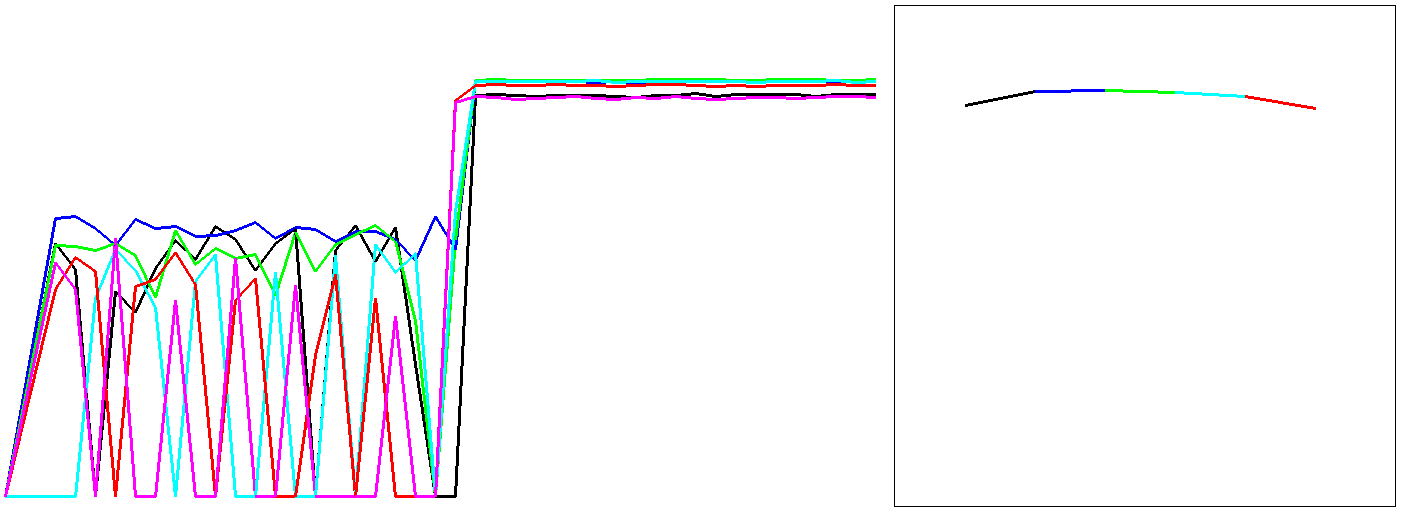
\includegraphics[width=\textwidth]{gui}
                \caption{Graphical user interface as an item is held in front of the scanner.}
                \label{fig:gui}
            \end{figure}
                
                \noindent In addition to reading numbers off the terminal, a Python script was made to produce a graphical user interface
                which displays values over time in real time. \Cref{fig:gui} shows a screenshot of the interface. The left portion is values
                from different LEDs over time, and the right portion shows an average of the last 20 readings, for each LED, to see if different
                items produce different waveforms. The screenshot is taken after an item got placed in front of the scanner, which is why the curves
                on the left go from low to high. This script was also used to record values, used to compare different materials, for later use.
                The interface has no values or axis labels, because it has simply been used to quickly verify the incoming data in real time.

    \section{Discussion}

            This section will discuss some design choices made, as well as an issue encountered with calibration,
            and some potential improvements to the project.
        
        \subsection{Speed}
            
            This application takes 10 SPS from the ADC, which is the slowest setting. In addition to this, is has has some delays between the readings, and
            discards one reading for every reading that is kept. It runs quite slowly. If this is to be used for some real-world
            application, efforts should be made to make the scanner faster, while still providing reliable data. This would require
            some trial and error, but would lead to a better product.

        \subsection{Low-dropout regulator}

            The NAU7802 has an option to use an LDO. 
            The code being mimicked, written for an Arduino \cite{arduinocode}, configures the LDO but
            doesn't enable it. Had the LDO been used, the values coming from the ADC may have been different. They are
            however only compared to other values from the same scanner, and the most important thing is to have the same settings
            across all readings.

        \subsection{Gain calibration}

            As stated in the user manual \cite{nau}, upon power-up, calibration routines should be executed, and it should be
            checked wether or not they return an error. The \textit{Gain calibration system} routine has returned an error every time
            it has been tested. It has been tested with various values for gain, and in various places in the code, never successfully.
            The Arduino code \cite{arduinocode} does not use this calibration routine. Due to it consistently failing, and the readings
            from the ADC being usable regardless, this calibration routine has been omitted from the application.

        \subsection{Interrupts vs. polling}

            After the ADC has made a conversion, it raises a flag saying that it is ready.
            This flag is accessible in a register via I$^2$C, but also on its own GPIO pin (DRDY).
            Our implementation polls the register to check for the flag after a
            after a conversion has been requested. This is not the best solution, because it
            keeps the processor busy while waiting for a conversion, and consumes power
            unnecessarily. This application uses polling because it is fast and easy to implement. It is
            not a problem in our application because there is no reason to save power, and the
            processor does not have anything else it could be doing while waiting. An interrupt
            routine would have been a better solution.
    \clearpage
    \section{Conclusions}
            
            This report has shown how the NAU7802 analog-to-digital converter has been implemented in the plastic scanner.
            It has looked at configuration, control and practical use.
            It has been shown that the implementation works as intended, but that it has room for improvements. It can be
            made to run faster, in order to be more suited for a real world application.
            This application uses polling to see if the ADC has a conversion ready. This occupies the processor
            unnecessarily, as well as uses more power than necessary.
            An interrupt routine would be a better solution.
            

    \clearpage
    \addcontentsline{toc}{section}{References}  
    \bibliographystyle{IEEEtran}
    \bibliography{bibliography}

\end{document}